\section{Support Vector Machine}
Per l'addestramento del modello è stato utilizzato il package R 
\texttt{e1071}.

\subsection{Holdout}
Le misure di accuracy, precision, recall e F-measure sono mostrate in 
Tabella \ref{tab:svm_h_performance}.

\begin{figure}[H]
	\centering
	\begin{tabular}{lcccc}
		\toprule
		& \textbf{Accuracy} & \textbf{Precision} & \textbf{Recall} & 
		\textbf{F-Measure}  \\
		\midrule
		Training	& 93,02\% & 75,17\% & 24,86\% & 37,37\%    	\\ 
		Validation	& 92,85\% & 70,89\% & 22,61\% & 34,29\%   	\\ 
		\bottomrule
	\end{tabular}
	\captionof{table}{Analisi performance con holdout}
	\label{tab:svm_h_performance}
\end{figure}

In Figura \ref{fig:svm_h_roc} sono mostrate le curve ROC per il training e il validation 
set.

\begin{figure}[H]
	\centering
	\begin{subfigure}[t]{1\textwidth}
		\begin{minipage}[t]{0.475\textwidth}
			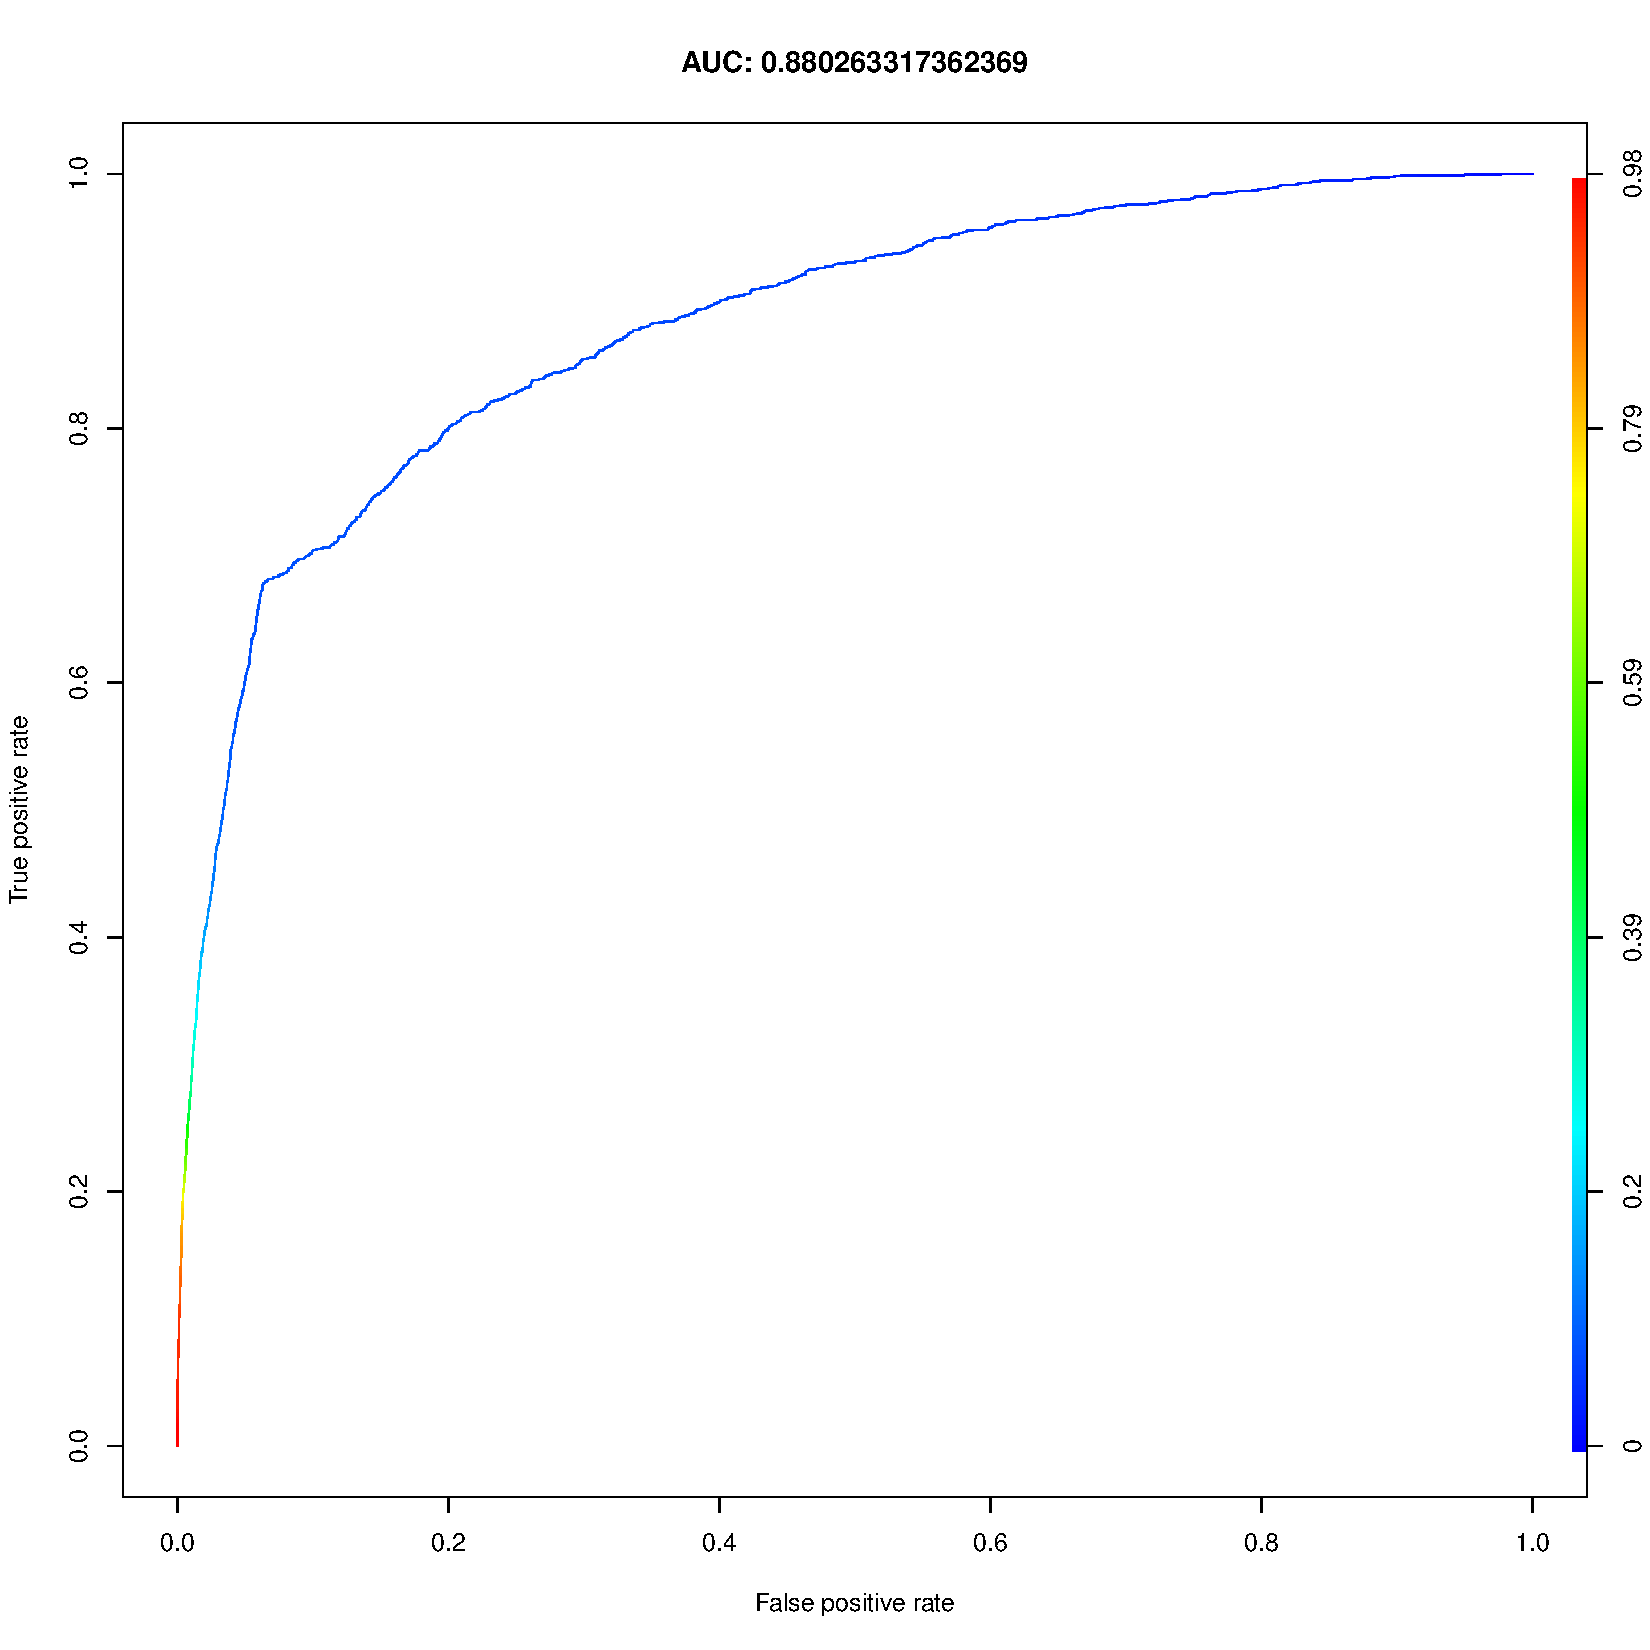
\includegraphics[width=\textwidth]{images/ml/svm/HoldoutSVM/auc_train}
			\captionof{figure}{Train ROC}
			\label{fig:svm_h_roc_train} 
		\end{minipage}
		\hfill
		\begin{minipage}[t]{0.475\textwidth}
			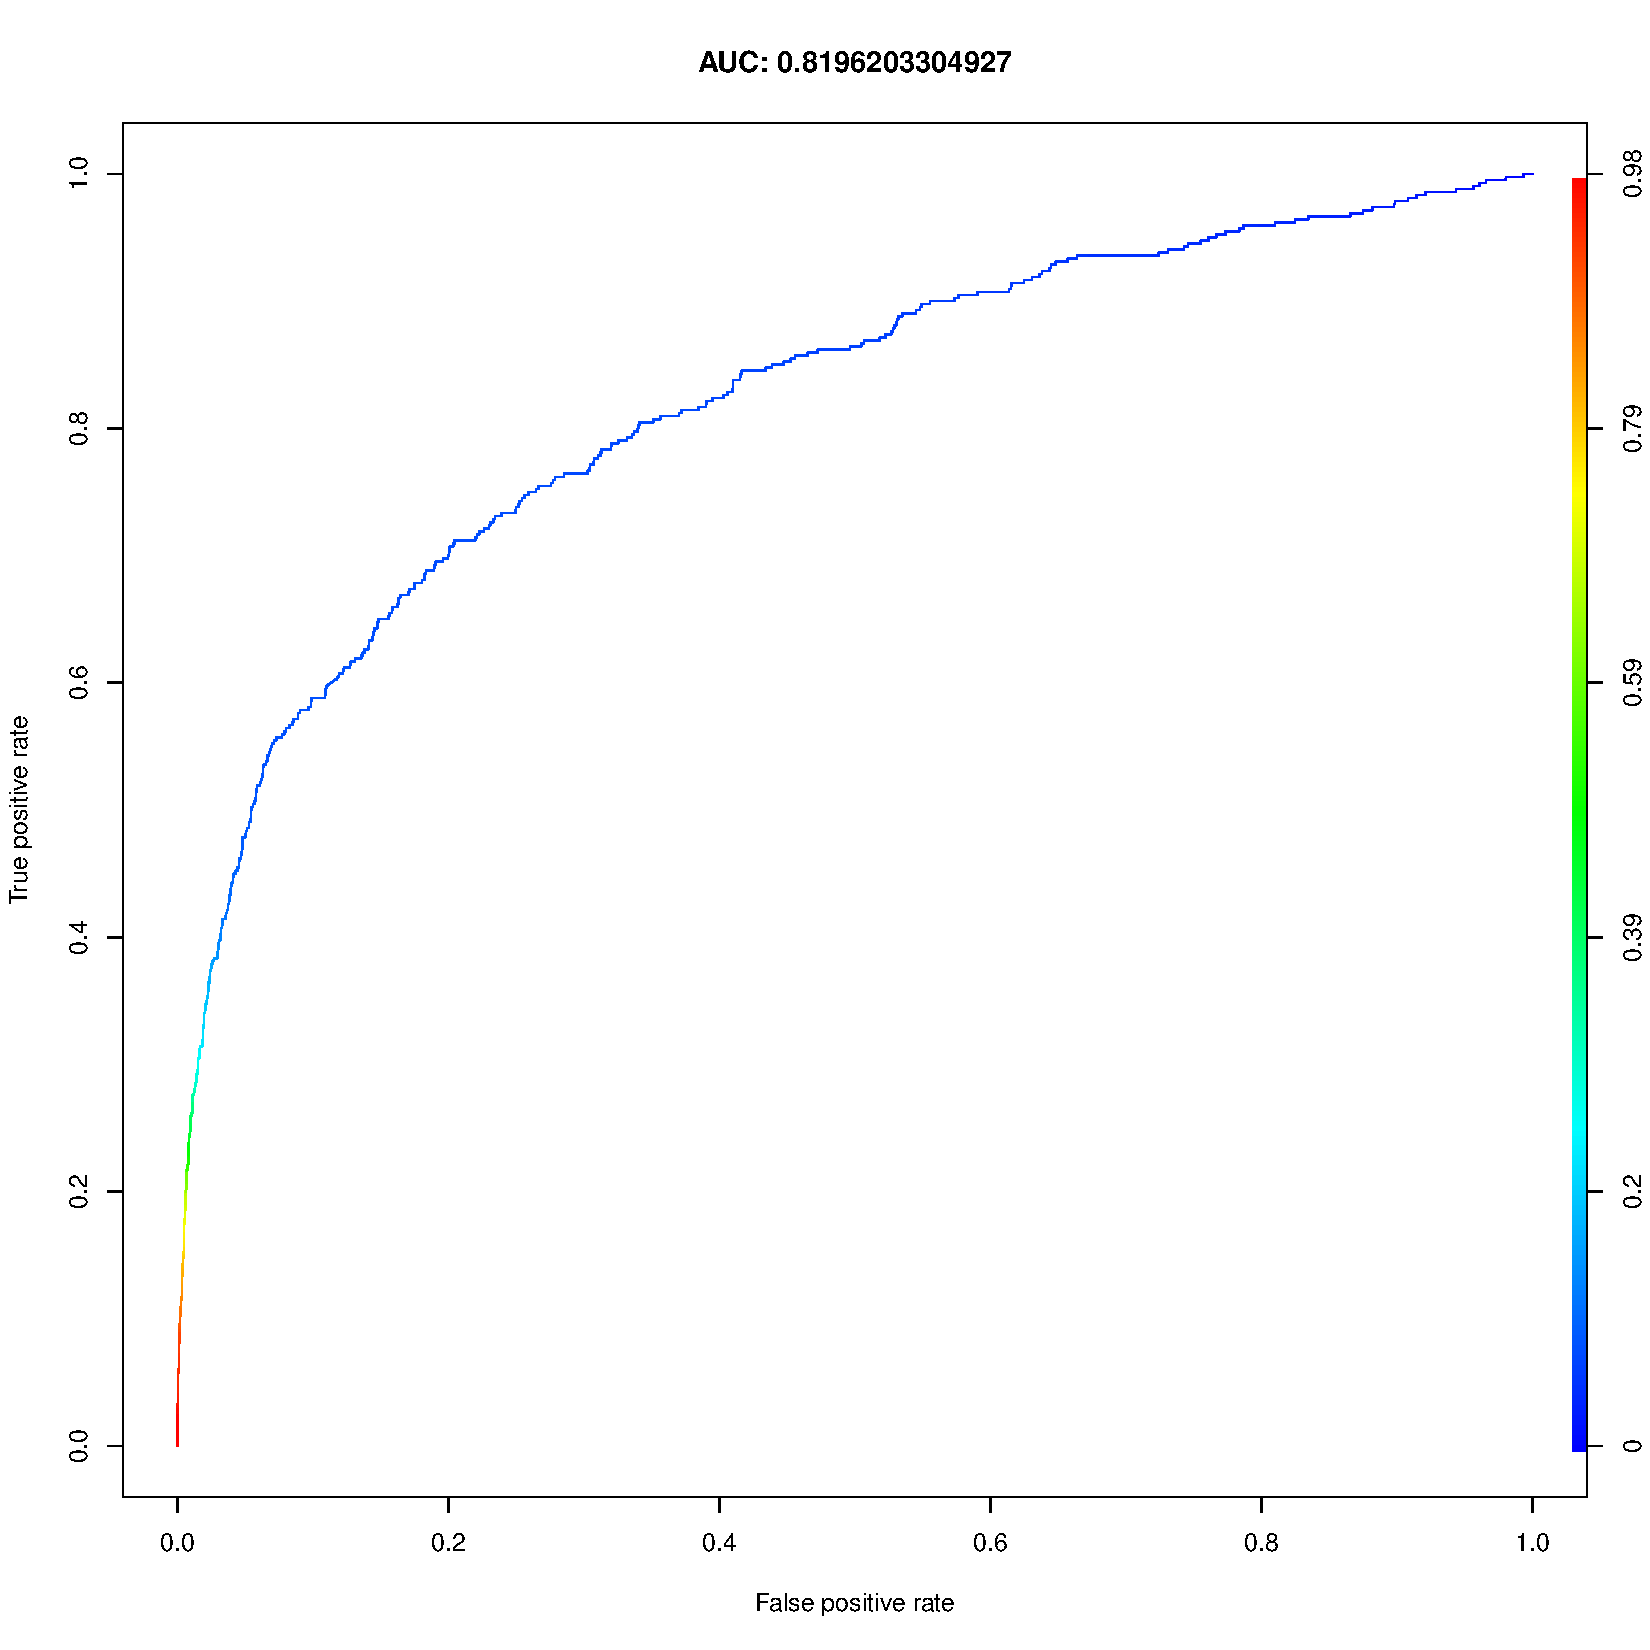
\includegraphics[width=\textwidth]{images/ml/svm/HoldoutSVM/auc_test}
			\captionof{figure}{Validation ROC}
			\label{fig:svm_h_roc_test} 
		\end{minipage}
	\end{subfigure}
	\caption{Curve ROC sul training e validation set}
	\label{fig:svm_h_roc}
\end{figure}

\subsection{10-fold Cross Validation}
Le misure finali di accuracy, precision, recall e F-measure sono state 
calcolare come la media delle misure su ogni fold. Vengono mostrate nella 
tabella \ref{tab:svm_cv_fold_performance} i dati relativi ad ogni fold e in 
tabella \ref{tab:svm_cv_performance} le misure complessive.

\begin{figure}[H]
	\centering
	\begin{tabular}{llcccc}
		\toprule
		&& \textbf{Accuracy} & \textbf{Precision} & \textbf{Recall} & 
		\textbf{F-Measure}  \\
		\midrule
		\multirow{10}{*}{Training} & Fold1 & 93,28\% & 76,90\% & 31,66\% & 
		44,85\% \\
		& Fold2 & 93,24\%  & 78,12\% & 30,56\% & 43,93\% \\
		& Fold3 & 93,28\%  & 77,73\% & 29,80\% & 43,08\% \\
		& Fold4 & 93,11\%  & 78,03\% & 30,01\% & 43,34\% \\
		& Fold5 & 93,46\%  & 77,92\% & 30,80\% & 44,14\% \\
		& Fold6 & 93,17\%  & 77,45\% & 30,71\% & 43,98\% \\
		& Fold7 & 93,63\%  & 76,31\% & 27,38\% & 40,30\% \\
		& Fold8 & 93,66\%  & 78,97\% & 28,41\% & 41,78\% \\
		& Fold9 & 93,66\%  & 78,61\% & 28,00\% & 41,29\% \\
		& Fold10 & 93,63\% & 77,58\% & 27,02\% & 40,08\%  \\
		\midrule
		\multirow{10}{*}{Validation} & Fold1 & 94,15\% & 78,57\% & 6,08\% & 
		11,28\% \\
		& Fold2 & 94,70\% & 60,00\% & 8,63\% & 15,08\% \\
		& Fold3 & 94,30\% & 80,00\% & 18,93\% & 30,61\% \\
		& Fold4 & 95,83\% & 62,06\% & 15,92\% & 25,33\% \\
		& Fold5 & 92,58\% & 64,28\% & 13,43\% & 22,21\% \\
		& Fold6 & 95,44\% & 66,66\% & 11,38\% & 19,44\% \\
		& Fold7 & 89,16\% & 66,66\% & 30,15\% & 41,52\% \\
		& Fold8 & 90,58\% & 75,43\% & 29,86\% & 42,78\% \\
		& Fold9 & 89,44\% & 59,62\% & 32,00\% & 41,64\% \\
		& Fold10 & 90,07\% & 72,60\% & 33,22\% & 45,58\% \\
		\bottomrule 
	\end{tabular}
	\captionof{table}{Analisi delle performance per ogni fold}
	\label{tab:svm_cv_fold_performance}
\end{figure}

\begin{figure}[H]
	\centering
	\begin{tabular}{lcccc}
		\toprule
		& \textbf{Accuracy} & \textbf{Precision} & \textbf{Recall} & 
		\textbf{F-Measure}  \\
		\midrule
		Training	&  94,412\% & 77,34\% & 29,43\%	& 42,67\%  	\\ 
		Validation	&  92,62\% & 68,50\% & 19,96\%	& 29,54\%	\\ 
		\bottomrule
	\end{tabular}
	\captionof{table}{Analisi performance complessive con cross validation}
	\label{tab:svm_cv_performance}
\end{figure}

Vengono infine mostrate in Figura \ref{fig:svm_cv_roc_valid} le curve ROC per ognuno dei fold sul 
validation set.

\begin{figure}[H]
	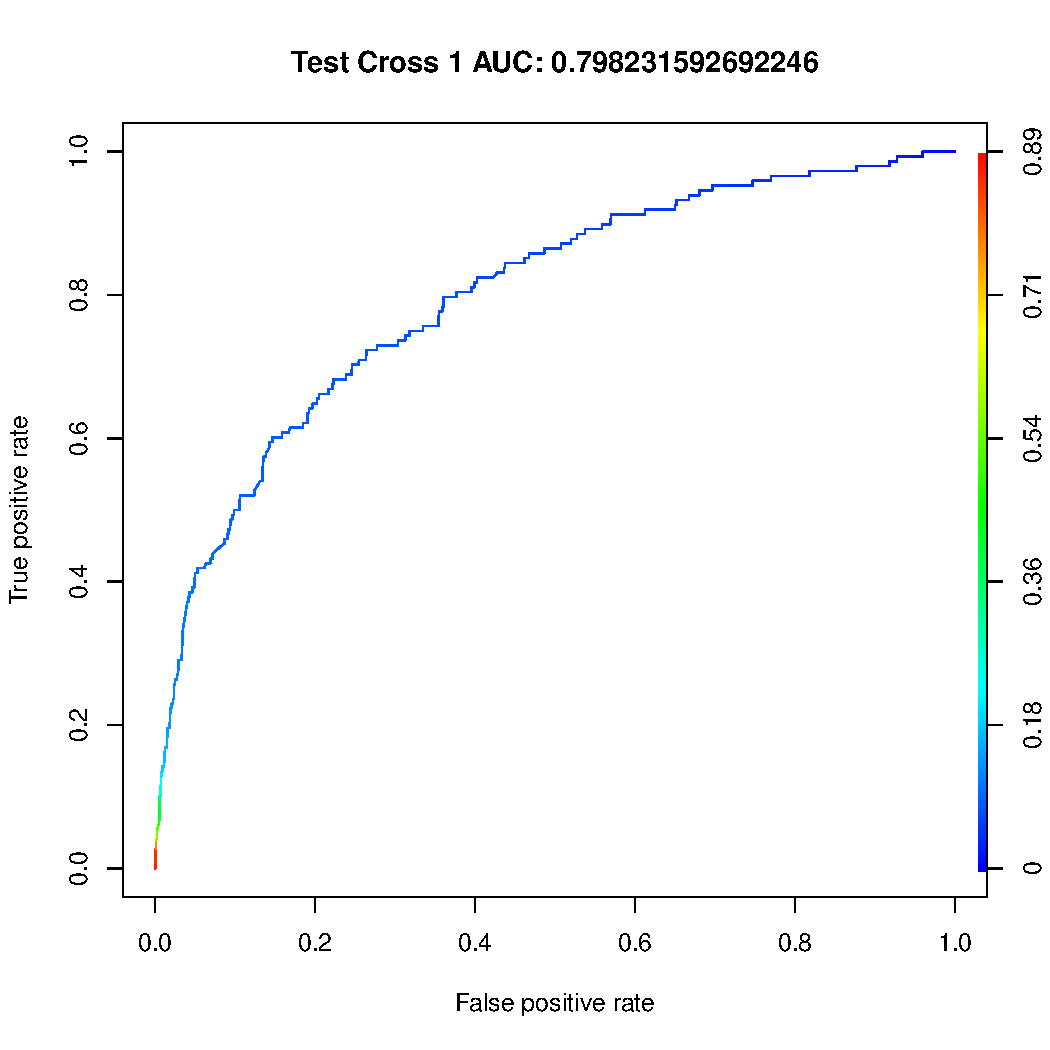
\includegraphics[width=.32\textwidth]{images/ml/svm/CrossValidationSVM/valid/auc_1}
	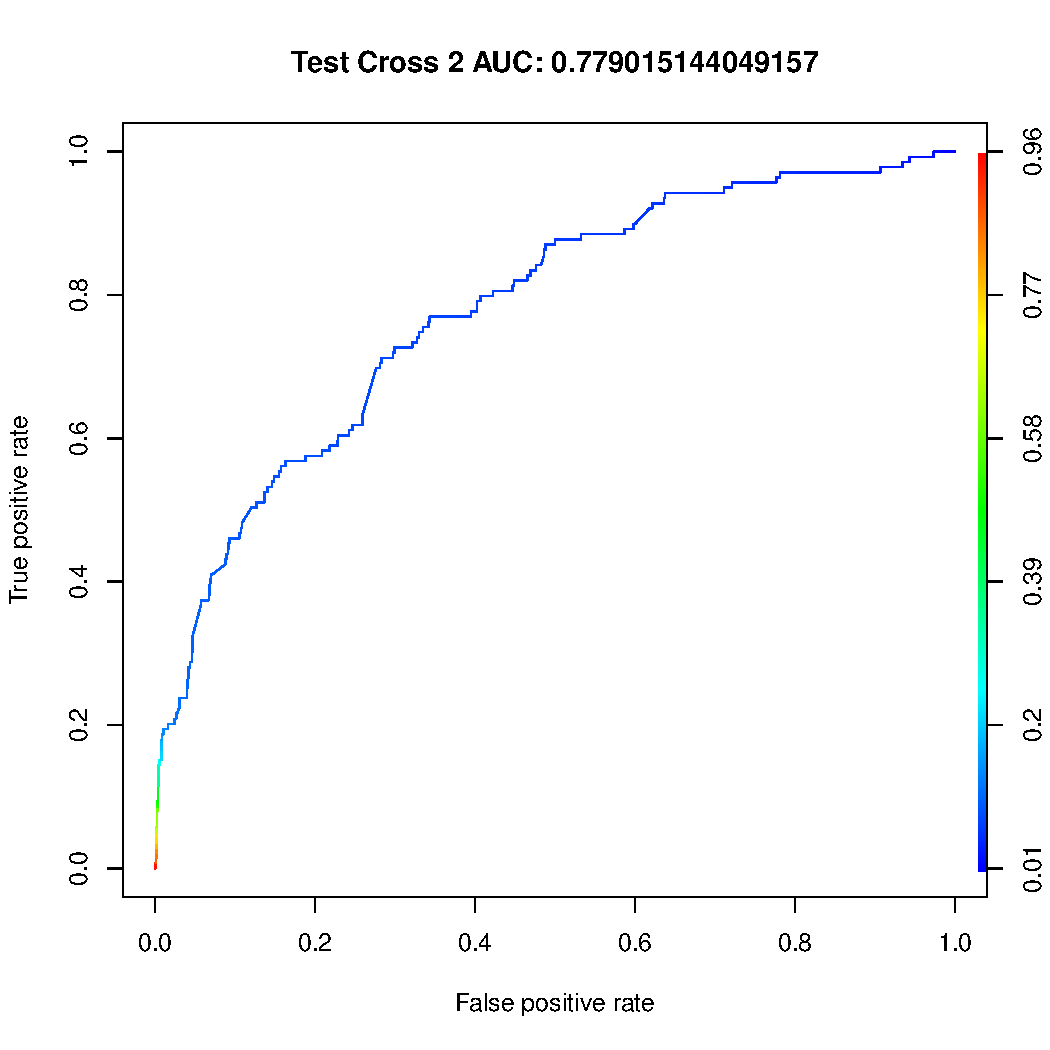
\includegraphics[width=.32\textwidth]{images/ml/svm/CrossValidationSVM/valid/auc_2}
	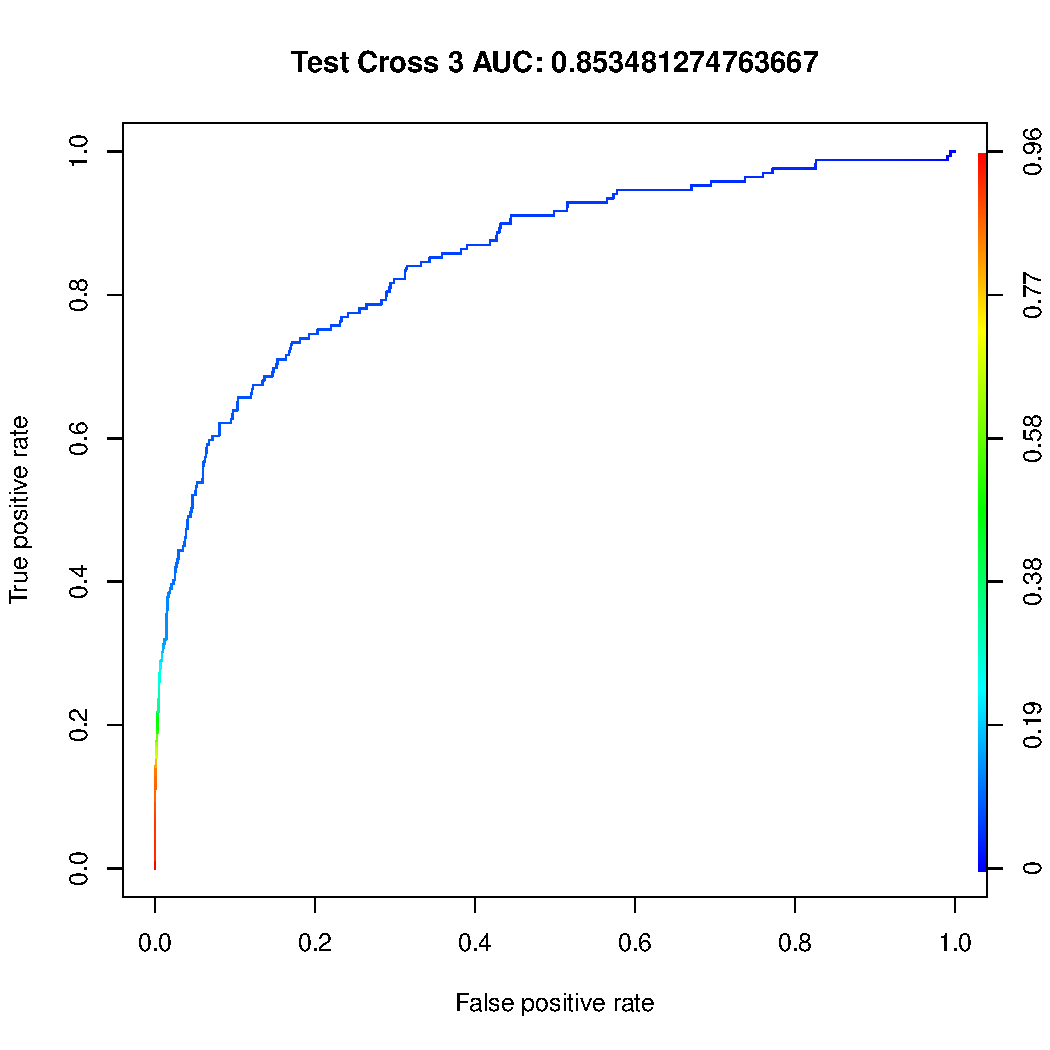
\includegraphics[width=.32\textwidth]{images/ml/svm/CrossValidationSVM/valid/auc_3}
	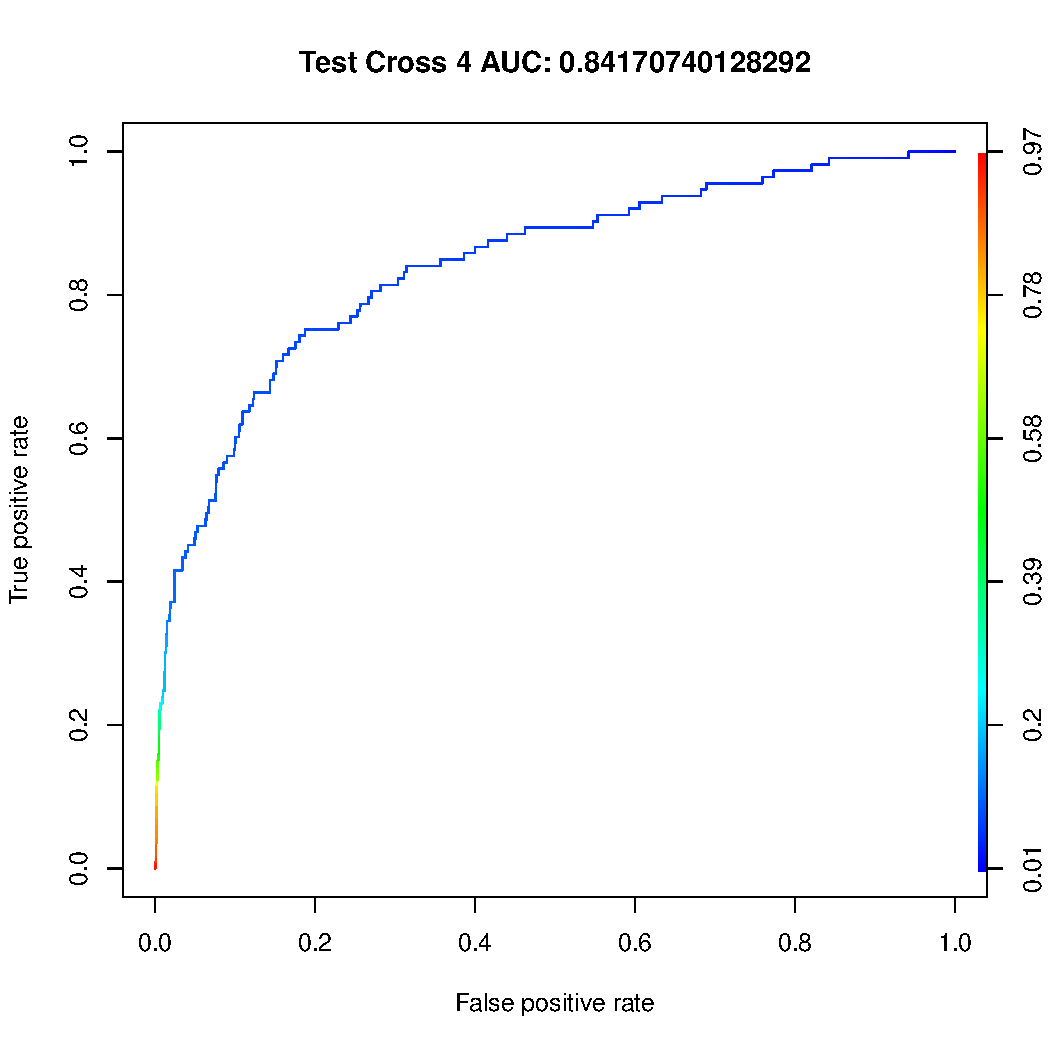
\includegraphics[width=.32\textwidth]{images/ml/svm/CrossValidationSVM/valid/auc_4}
	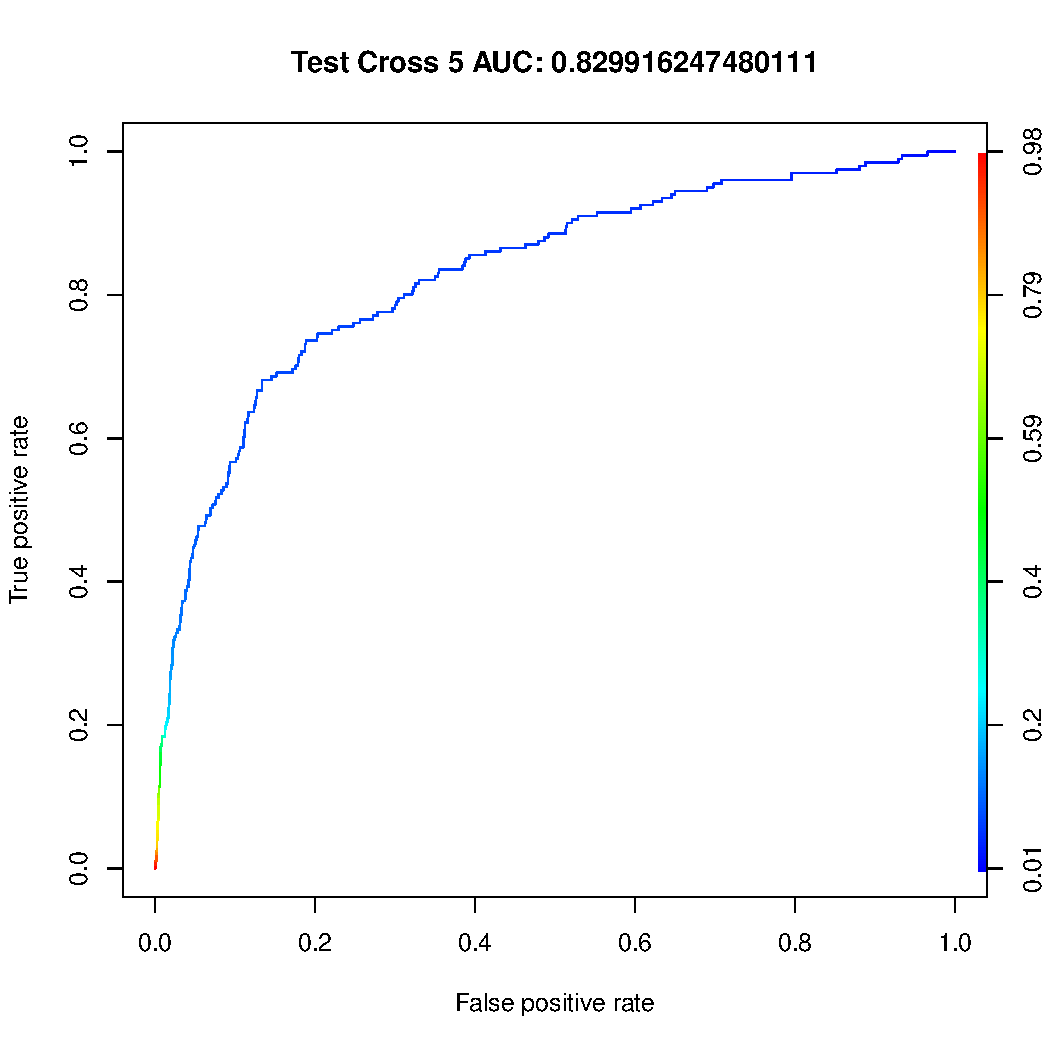
\includegraphics[width=.32\textwidth]{images/ml/svm/CrossValidationSVM/valid/auc_5}
	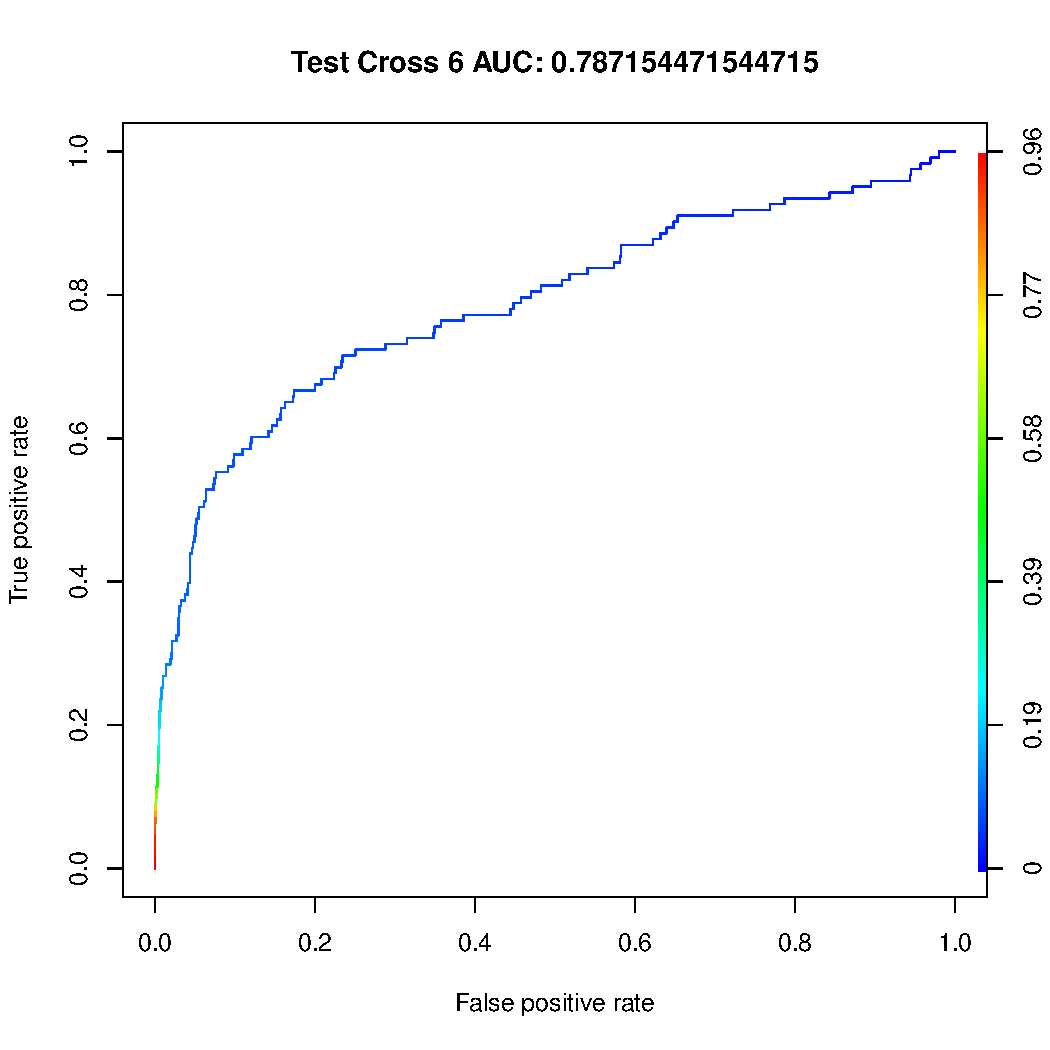
\includegraphics[width=.32\textwidth]{images/ml/svm/CrossValidationSVM/valid/auc_6}
	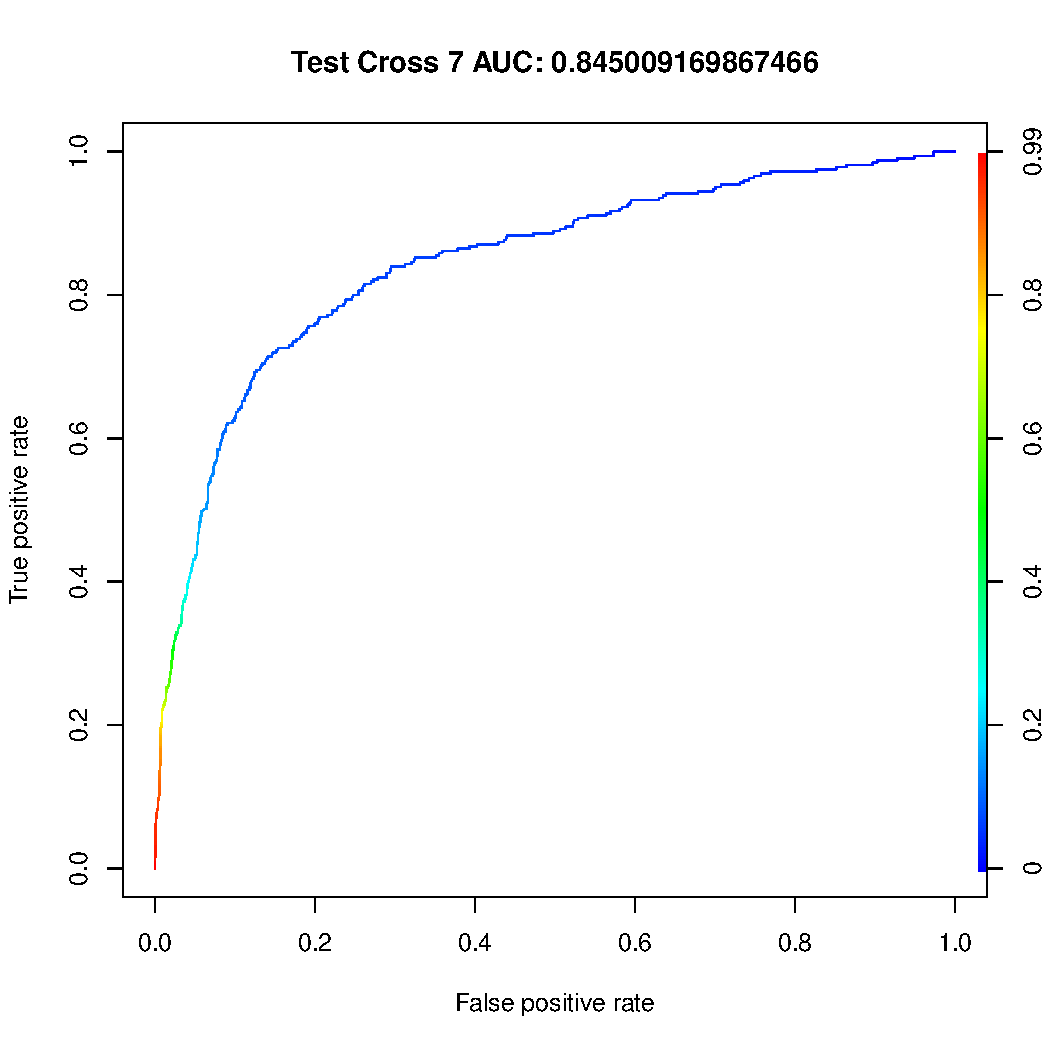
\includegraphics[width=.32\textwidth]{images/ml/svm/CrossValidationSVM/valid/auc_7}
	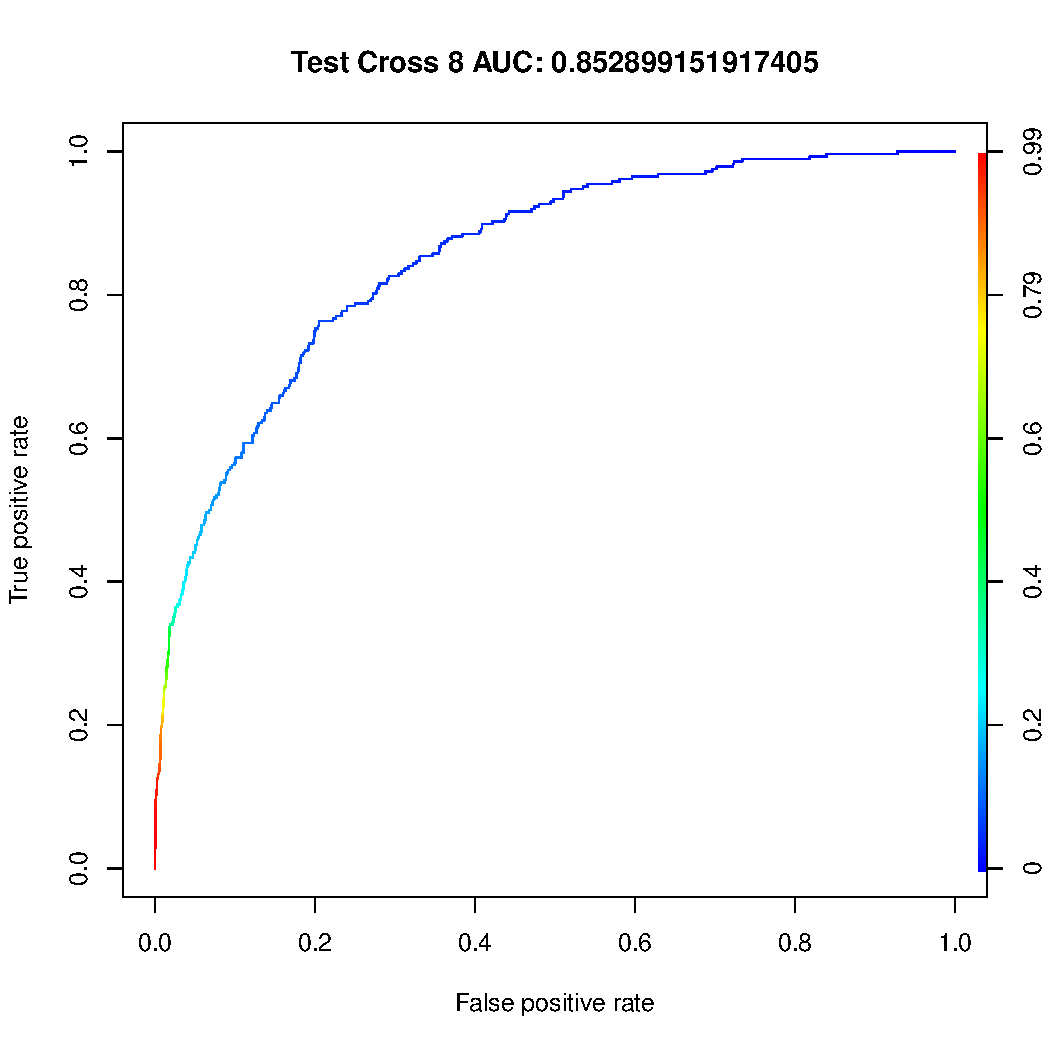
\includegraphics[width=.32\textwidth]{images/ml/svm/CrossValidationSVM/valid/auc_8}
	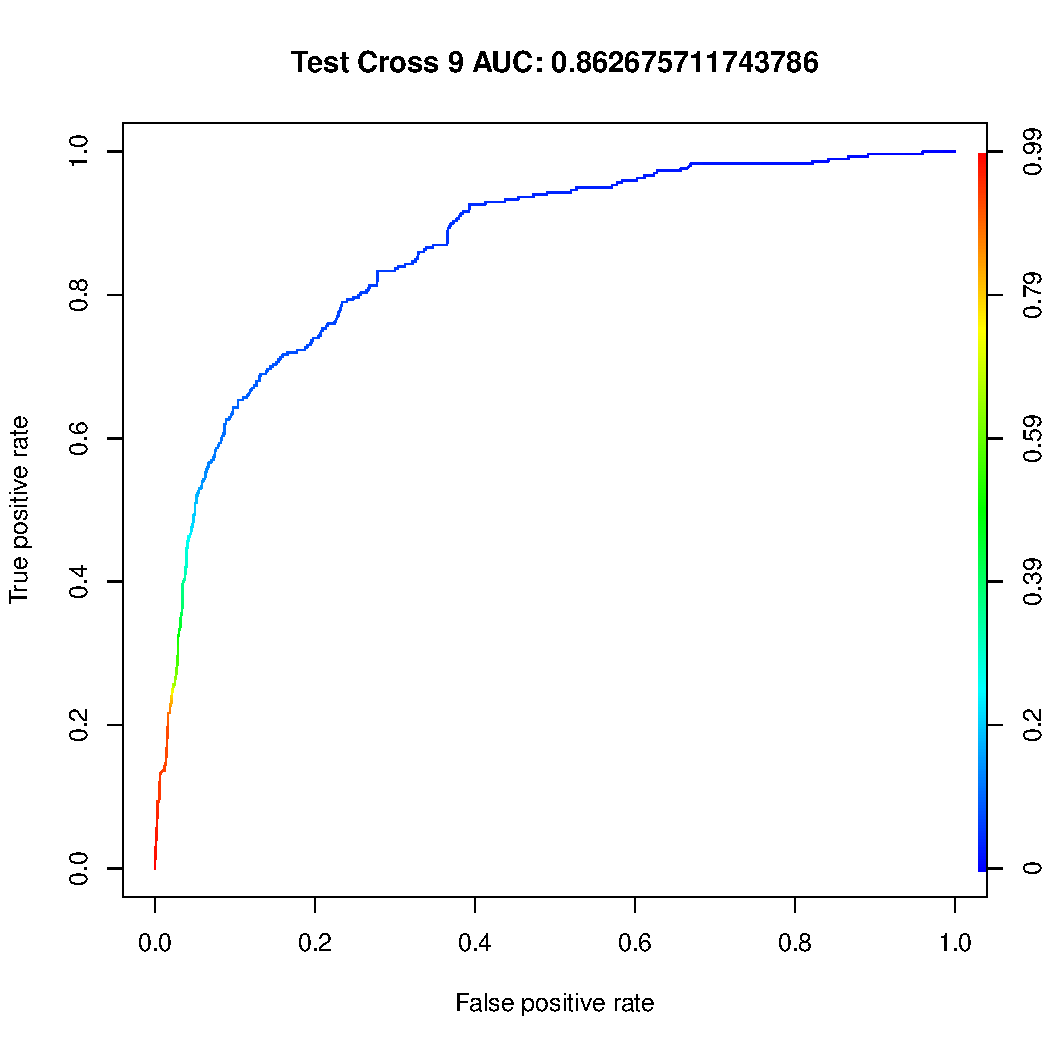
\includegraphics[width=.32\textwidth]{images/ml/svm/CrossValidationSVM/valid/auc_9}
	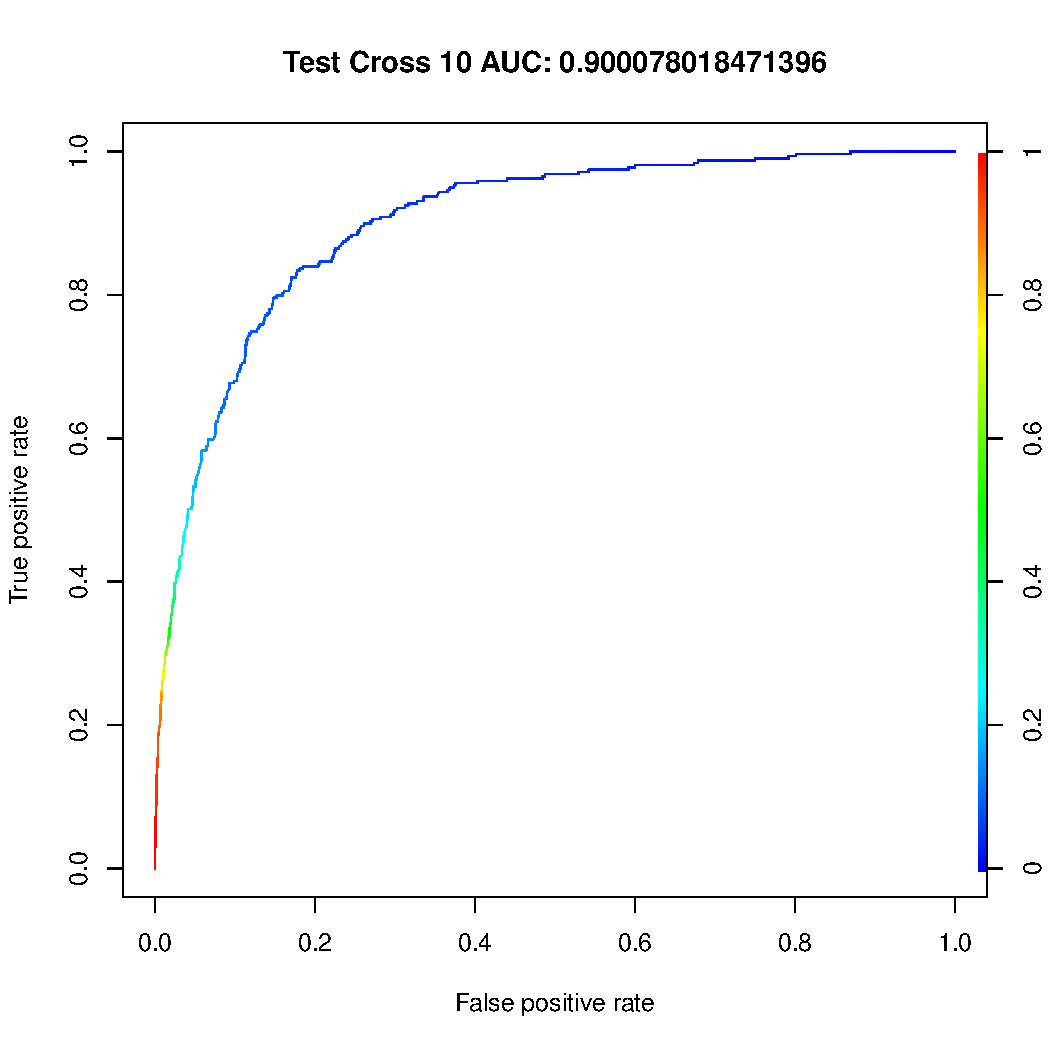
\includegraphics[width=.32\textwidth]{images/ml/svm/CrossValidationSVM/valid/auc_10}
	\caption{Curve ROC sul validation set}
	\label{fig:svm_cv_roc_valid}
\end{figure}
